\documentclass[11pt,conference]{IEEEtran}
\IEEEoverridecommandlockouts

% The preceding line is only needed to identify funding in the first footnote. If that is unneeded, please comment it out.
\usepackage{biblatex}
\addbibresource{refs.bib}

\author{Andreas Wenzelhuemer}
\usepackage{amsmath,amssymb,amsfonts}
\usepackage{algorithmic}
\usepackage{graphicx}
\usepackage{textcomp}
\usepackage{xcolor}
\usepackage{parskip}
\usepackage{listings}
\lstset{basicstyle=\scriptsize\ttfamily}

\def\BibTeX{{\rm B\kern-.05em{\sc i\kern-.025em b}\kern-.08em
    T\kern-.1667em\lower.7ex\hbox{E}\kern-.125emX}}
\graphicspath{ {./images/} }
\begin{document}
\title{CQS: Command Query Separation}

\maketitle

\begin{abstract}
This paper describes the architectural pattern Command and Query Separation (CQS) with it's advantages and disadvantages.
Additionally the so called Command and Query Segregation (CQRS) gets explained, which is based on CQS.
Further it includes an practical example in C\# and the MediatR library. 
\end{abstract}

\begin{IEEEkeywords}
CQS, CQRS, MediatR
\end{IEEEkeywords}

\section{Introduction}

Traditionally for a defined domain, a single model is used which handles all operations like read, update, create and delete.
However, as the model becomes larger and complexer, the code becomes more and more unmanageable.
For many operations it becomes unclear, if the method is returning data, modifies a state or does both.
This means there could always be side effects.
With the Command Query Separation (CQS) pattern, it is possible to separate each of these operations.

\section{CQS}

\subsection{What is CQS?}

The CQS pattern is a design principle that states that a method should either execute an action or return a value, but not both. This means that a method should either modify the state of a system or return a value, but not both. The purpose of CQS is to make it clear what the purpose of a method is and to ensure that it is used correctly.

One common way to implement CQS is to create two types of methods: commands and queries. Commands are methods that execute an action and do not return a value. Queries are methods that return a value but do not modify the state of the system. By clearly separating commands and queries, it becomes easier to understand the purpose of each method and to ensure that they are used correctly.

CQS can be useful in a variety of situations, including distributed systems, event-driven architectures, and microservices. It can help to improve the clarity and maintainability of code, and can make it easier to understand and reason about the behavior of a system~\cite{martinfowler-cqs}.

\begin{figure}[h]
    \centering
    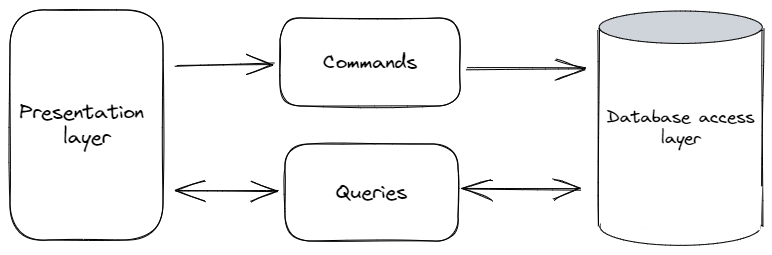
\includegraphics[width=0.5\textwidth]{images/CQS.png}
    \caption{CQS~\cite[14]{cqrs-in-practise}}
    \label{fig:cqs}
\end{figure}

\subsection{Advantages}

What are the actual benefits of Queries and Commands for each domain model instead of creating on larger logic class which combines all operations?~\cite{martinfowler-cqs}

\paragraph{Improved clarity and maintainability}
By clearly separating commands and queries, it becomes easier to understand the purpose of each method and to ensure that they are used correctly. This can make the code more maintainable and easier to understand.

\paragraph{Improved testability}
By separating commands and queries, it becomes easier to write unit tests that focus on either the action being performed or the value being returned, rather than both at the same time. This can make it easier to write tests that are more focused and effective.

\paragraph{Improved scalability}
CQS can make it easier to scale a system, because the command and query models can be optimized independently. For example, the command model may need to support high write throughput, while the query model may need to support high read throughput. By separating these concerns, it is possible to optimize each model for its specific workload.

\paragraph{Improved flexibility}
By separating commands and queries, it becomes easier to make changes to the system without affecting the other. For example, it is possible to change the implementation of the command model without affecting the query model, or vice versa. This can make it easier to evolve the system over time.

\paragraph{Improved consistency}
 By separating the responsibility for reading and writing data, it becomes easier to ensure that the data is consistent across the system. For example, it is possible to use eventual consistency or other techniques to ensure that the data in the query model is up-to-date with the data in the command model.

\subsection{Disadvantages}

CQS can be useful pattern for improving the separation of concerns in a codebase and making it easier to reason about the behavior of individual methods or functions, but it is not without problems and disadvantages.

One disadvantage would be, that you need a lot more classes.
For each operation multiple classes have to be created.
Each handler, query or command itself are simple and easy to understand, but the project structure itself gets more complicated.
In contrast to the classic approach where all operations are combined in one class.
Especially for new developers CQS could add additional complexity.

Also operations like pop() for stacks wouldn't be possible with CQS because it would be a command which also returns something.
Instead one command and one query have to be called.

\subsection{Challenges and Best Practices}

There are a few challenges and best practices to consider when implementing Command Query Separation (CQS)~\cite{martinfowler-cqs}.

Avoiding confusion: One challenge with CQS is that it can be confusing to determine which methods should be commands and which should be queries. A good rule of thumb is to ask yourself whether the method is changing the state of the system or simply returning data. If the method is changing the state of the system, it should be a command; if it is returning data, it should be a query.

Testing commands and queries separately: It is important to test commands and queries separately to ensure that they are working correctly. This can be done by using mock objects to simulate the effects of the commands or by using test data to verify the results of the queries.

Handling errors: Another challenge with CQS is handling errors that may occur when executing commands. It is generally a good idea to use try-catch blocks or other error-handling techniques to ensure that errors are properly handled and do not cause the system to crash.

Keep commands and queries small: To make it easier to understand and maintain the code, it is generally a good idea to keep commands and queries small and focused on a single responsibility. This can also help to reduce the risk of introducing bugs by limiting the scope of changes to a single method.

Documenting the separation: It can be helpful to document the separation of commands and queries in the code or in external documentation to make it easier for other developers to understand the intended purpose of each method.

Overall, the key to successfully implementing CQS is to carefully consider the responsibilities of each class and to clearly separate the commands from the queries to ensure that each class has a single, well-defined responsibility.

\subsection{Area of application}

Here are some examples in which kind of projects or architectures CQS can be used.

\begin{itemize}
    \item {Web applications: CQS can be used to separate HTTP request methods. POST, PUT, DELETE would be commands while GET would be a query.}
    \item {Database systems: INSERT, UPDATE, DELETE operations could be handled separately from read operations such as SELECT.}
    \item {Event driven architectures: Operations, that generate events (commands) could be separated from those that consume events (queries). This could help improve the decoupling and flexibility of the system.}
\end{itemize}

\section{CQRS?}

\subsection{What is CQRS?}
CQRS (Command Query Responsibility Segregation) is a pattern that is based on CQS and takes it a step further by separating the responsibility for reading and writing data into separate components or models. In a CQRS system, the model responsible for writing data is known as the Command Model, and the model responsible for reading data is known as the Query Model.

The main benefit of using CQRS is that it allows the read and write models to be optimized independently, which can lead to improved performance and scalability. It can also make it easier to evolve the system over time by allowing changes to be made to one model without affecting the other.

It is possible to use separate databases for read and write operations in a CQRS system. This can be useful if the read and write workloads have very different requirements in terms of performance, scalability, or data consistency.

For example, the write database may need to support high write throughput and data integrity, while the read database may need to support high read throughput and low latency. By using separate databases, it is possible to optimize each database for its specific workload and improve the overall performance of the system.

That being said, it is not strictly necessary to use separate databases in a CQRS system. It is possible to use a single database and partition the data in some other way, such as using different tables or schemas for the read and write models. The choice of whether to use separate databases or not will depend on the specific requirements and constraints of the system~\cite{martinfowler-cqrs}.

\begin{figure}[h]
    \centering
    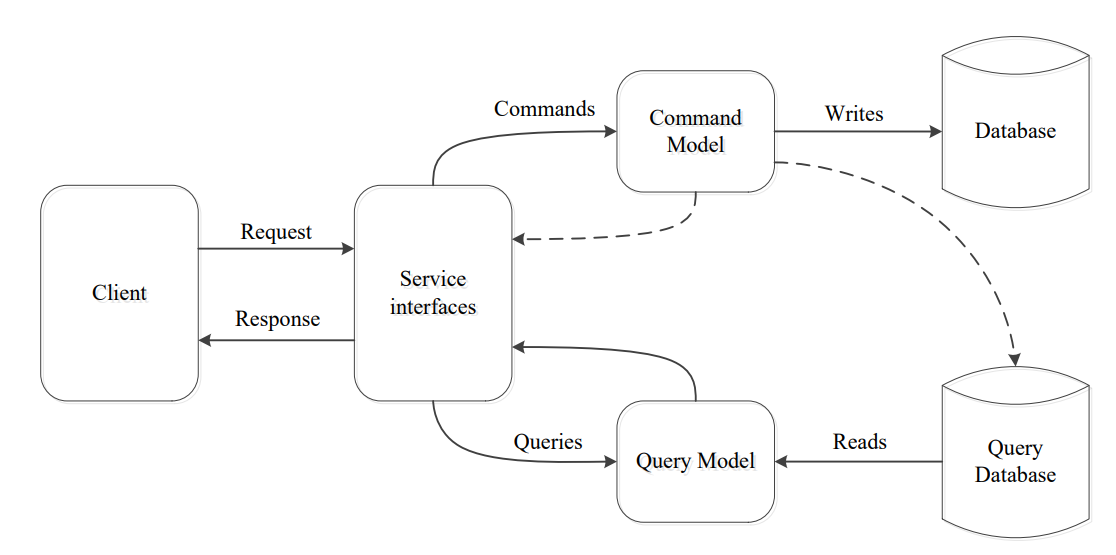
\includegraphics[width=0.5\textwidth]{images/CQRS.png}
    \caption{CQRS~\cite[15]{cqrs-in-practise}}
    \label{fig:cqrs}
\end{figure}

\subsection{When to use it}

You might consider using CQRS instead of CRUD in situations where you need to support a high level of read and write performance, or where the requirements for reading and writing data are significantly different. For example, if you have a system that needs to support high levels of read traffic (e.g., a social media platform that needs to display real-time updates to users), you might use CQRS to separate the read and write workloads in order to improve performance. Alternatively, if you have a system where the requirements for reading and writing data are significantly different (e.g., a system that requires complex data transformations or validation rules for writes, but simple data retrieval for reads), you might use CQRS to better encapsulate these distinct responsibilities~\cite{martinfowler-cqrs}.

Overall, CQRS can be a useful pattern in certain situations where the requirements for reading and writing data are significantly different, or where you need to support high levels of read and write performance. However, it can also add complexity to a system, and should be carefully considered in the context of the specific requirements of a project~\cite{martinfowler-cqrs}.

\section{The connection with SOLID Principles}

The SOLID principles are a set of guidelines for designing software that is easy to maintain and extend over time.
One of the SOLID principles is the Single Responsibility Principle (SRP), which states that a class should have only one reason to change. In other words, a class should have a single, well-defined responsibility.
Command Query Separation (CQS) is a principle that is related to the Single Responsibility Principle. It states that every method in a class should either be a command that performs an action or a query that returns data, but not both~\cite{solid-principles}.

CQS is used to help ensure that a class has a single responsibility and follows the Single Responsibility Principle. By separating commands and queries into separate methods, it becomes easier to understand the purpose of each method and the responsibilities of the class as a whole.
For example, consider a class that is responsible for managing a user account. A command method might be "updatePassword," which changes the password for the user account. A query method might be "getUsername," which returns the username for the user account. By following CQS, it is clear that the class is responsible for managing the user account and its associated data, but not for performing actions on that data (which would be the responsibility of another class).

In summary, CQS is a principle that helps to ensure that classes have a single, well-defined responsibility, which is an important aspect of the Single Responsibility Principle in the SOLID principles.

\section{Implementation of CQS with MediatR and C\#}

\subsection{What is a Mediator?}

A mediator is a design pattern that allows you to decouple the components of a system by introducing a middleman that handles the communication between the components.

\subsection{What is the MediatR library?}

MediatR is a popular mediator library implemented in C\#.

MediatR can be used to implement the CQS pattern by separating commands and queries into distinct classes, and using MediatR to handle the routing and execution of these messages. For example, you might define a command class to represent a request to update a database record, and a query class to represent a request to retrieve data from the database. You can then use MediatR to handle the routing of these requests to the appropriate handler classes, which can be responsible for executing the actual command or query.

MediatR can be a useful tool for implementing the CQS pattern in a .NET application, as it provides a lightweight and flexible framework for building message-based systems~\cite{mediatr}.

The library can be registered using .NET Core dependency injection.
After the registration the \texttt{IMediator} interface can injected into controllers or azure functions using constructor injection.

\subsection{Example with Azure Functions}

We have a database with different heroes and want read and write operations for them over separate microservices.
One possibility would be to use the CQS pattern, which we will use here.

First each operation will be one separate microservice:

\begin{itemize}
    \item {HeroesGetAll: Get all heroes}
    \item {HeroesGetOne: Get one hero by id}
    \item {HeroesPost: Insert new hero}
    \item {HeroesPut: Update existing hero}
\end{itemize}

Each operation is implemented as a serverless azure function.
Depending on the operation, a query or command is needed.
For commands additional validators and checks are needed.

First the MediatR package needs to be installed and configured.
.NET Core has a built in dependency injection container.
MediatR can be registered by calling the method \texttt{AddMediatR()}.
After that MediatR can be injected everywhere where needed using constructor injection.

\begin{lstlisting}[caption=Register MediatR]
public override void Configure(
    IFunctionsHostBuilder builder)
{
    builder.Services.AddMediatR();
}
\end{lstlisting}

With \texttt{mediator.send(..)} a command or query can be sent to the mediator.
In the example below an azure function was created.
First a new query object gets created, which gets passed to the mediator.
The mediator routes the object to a corresponding registered handler, executes it and returns the response to the caller.
In case of an exception, the appropriate status code with message gets returned.

\begin{lstlisting}[caption=Azure Function with MediatR]
[FunctionName("Heroes_GetOne")]
public async Task<IActionResult> Run(
    [HttpTrigger(AuthorizationLevel.Function,
    RouteConfig.GET,
    Route = RouteConfig.URL_ID)]
    HttpRequest request,
    Guid id)
{
    try
    {
        var query = new GetHeroByIdQuery(id);
        var response = await mediator.Send(query);
        return new OkObjectResult(response);
    }
    catch (NotFoundException ex)
    {
        return new NotFoundObjectResult(ex.Message);
    }
    catch (Exception ex)
    {
        logger.LogError(ex.Message);
        throw;
    }
}
\end{lstlisting}

The command or query needs to derive from IRequest.
Here you can see an example of an query with one parameter.
The response in this case is an HeroDto.

\begin{lstlisting}[caption=Query]
public class GetHeroByIdQuery : IRequest<HeroDto>
{
    public GetHeroByIdQuery(Guid id)
    {
        Id = id;
    }

    public Guid Id { get; init; }
}
\end{lstlisting}

The handler contains the implementation for one query or command.
There should exist only one handler for each query or command.

\begin{lstlisting}[caption=Query Handler]
public class GetHeroByIdQueryHandler
    : IRequestHandler<GetHeroByIdQuery, Dto>
{
    public async Task<HeroDto> Handle(
        GetByIdQuery request,
        CancellationToken _)
    {
        var entity = await dbContext.Heroes
                        .FindAsync(request.Id);

        if (entity is null)
            throw new NotFoundException();

        return new HeroDto(entity.Id, entity.Name);
    }
}
\end{lstlisting}

It is also possible to add validation by using FluentValidation, a common validation package.
In the example underneath, a name can't be null or empty and needs to contain a minimum length of 5 characters.

\begin{lstlisting}[caption=Validator]
public class CreateCommandValidator  
        : AbstractValidator<CreateCommand>
{
    public CreateCommandValidator()
    {
        RuleFor(x => x.Name)
            .NotNull()
            .NotEmpty()
            .MinimumLength(5);
    }
}
\end{lstlisting}

In total these would be the classes we would need for the operations specified above.

\begin{itemize}
    \item {CreateHeroCommand}
    \item {CreateHeroCommandHandler}
    \item {CreateHeroCommandValidator}
    \item {UpdateHeroCommand}
    \item {UpdateHeroCommandHandler}
    \item {UpdateHeroCommandValidator}
    \item {GetHeroByIdQuery}
    \item {GetHeroByIdQueryHandler}
    \item {GetHeroesQuery}
    \item {GetHeroesQueryHandler}
\end{itemize}

These should highlight the difference to a classic architecture where you would have one \texttt{IHeroService} and \texttt{HeroService}.
The class would include all necessary operations, nothing else is needed.
For this few simple operations, the \texttt{HeroService} would be enough, but it could become extremely complex with more operations which are often not as straight forward as these standard operations.

\section{Conclusion}

In conclusion, using Command Query Separation (CQS) can help to improve the design and maintainability of software by ensuring that classes have a single, well-defined responsibility. By separating commands and queries into separate methods, it becomes easier to understand the purpose and responsibilities of each class, and to make changes to the code without affecting unrelated functionality.

CQS can also help to improve the testability of software by making it easier to test individual methods in isolation. It can also reduce the risk of introducing bugs by limiting the scope of changes to a single method.

MediatR seems to be the de facto standard for implementing CQS in C\#.
It is very easy to use and to configure and works very well.

One thing to consider when implementing CQS is the increased overall complexity of the project.
For each class a query or command, a handler and sometimes additionally a validator is needed.
Instead with the classic approach you have one service or logic class with all the operations in one file.

Overall, the use of CQS can lead to more modular, flexible, and maintainable software that is easier to understand and modify over time.
It definitely makes sense in certain use cases and is definitely good to have the concept in the back of your mind.

\printbibliography

\end{document}
